\chapter{Example Data Processing}

This chapter is partly a show case of results that are possible with
Ames Stereo Pipeline. Yet it is also a shortened guide that shows the
commands and stereo.default files used to process data. It can be hard
try to figure out what settings to start with and hopefully this will
provide starting point ideas.

\section{Guidelines for Selecting Stereo Pairs}

When choosing image pairs to process, images that are taken with
similar viewing angles, lighting conditions, and significant surface
coverage overlap ($\sim80$\% is ideal) are the best suited for
creating terrain models from. Depending on the characteristics of
the mission data set and the individual images, the degree of
acceptable variation will differ. Significant differences between
image characteristics increases the error propagated through to the
resulting data products.

Images do not need to be map projected before running the \texttt{stereo}
program. That being said, for images which contain large topographic
variation (and therefore large disparity differences across the
scene--think Valles Marineris), sometimes map-projecting the images
can help, as it sometimes improves the correlation (at least until
we get our adaptive correlation window strategies in place).  However,
be careful about map-projecting.  For example, the HiRISE RDR
products, which are map projected, have been map-projected onto a
smoothed MOLA terrain model, so these images are not suitable for
stereo processing, because the act of projecting them on to a terrain
model introduces disparity into the source images that will lead
to poor results.

The images should be photometrically calibrated (in whatever fashion
suits your purposes), as excessively noisy images will not correlate
well.  If there are photometric problems with the images, those
photometric defects could be misinterpreted as topography.

The Stereo Pipeline can deal with arbitrary images with accompanying
camera information, but doing so requires a significant amount of
extra work and setup which are not covered in this document, and
are considered `advanced usage.'  The image type that is easiest
for the user to provide and for the Stereo Pipeline's \texttt{stereo}
program to ingest are ISIS 3 cube files (\texttt{.cub}).  In order
for \texttt{stereo} to utilize the detailed camera data available
for planetary data (SPICE), the images must have had ISIS's
\texttt{spiceinit} program run on them.

\section{Apollo 15 Metric Camera Images}

Apollo Metric images were all taken at regular intervals, that means
that the same stereo.default can be used for all sequential pairs of
images. Apollo Metric images are some of easiest images to make stereo
data from.

The scans performed by ASU are so detailed that the film grain can be
made out. This detail of information is not helpful for the
correlator, so it is recommended that subsampling the image by 4 so an
actual signal is available at 1 px samplings.

Currently the tools to ingest Apollo TIFFs into ISIS are not
available.

\subsection{Ansgarius C}

Ansgarius C is a small crater on the west edge of the farside of the
Moon, near the equator. It is east of Kapteyn A and B.

\subsubsection*{Screenshot}

\begin{figure}[h!]
\centering
  \subfigure[{\tt 3D Rendering}]{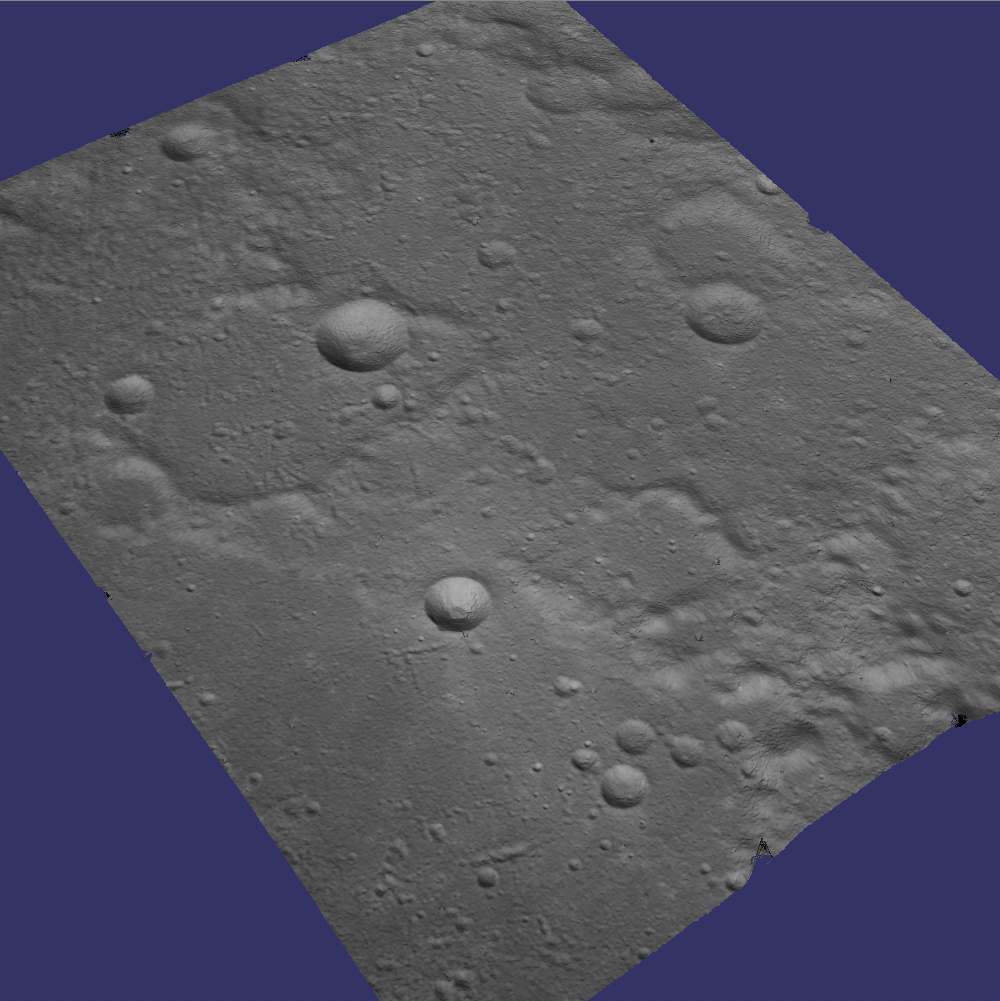
\includegraphics[width=3in]{images/examples/metric/metric_example.png}}
  \hfil
  \subfigure[{\tt KML Screenshot}]{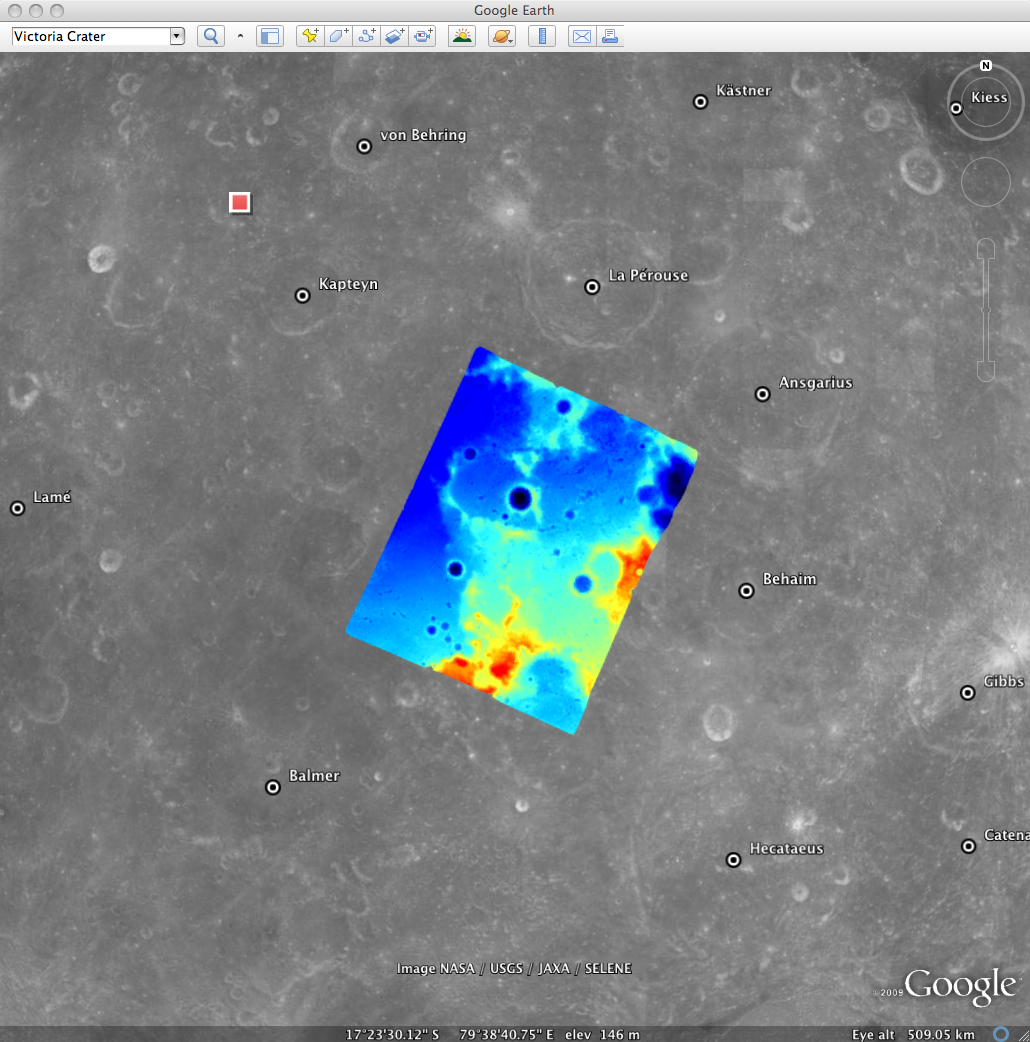
\includegraphics[width=3in]{images/examples/metric/metric_ge_example.png}}
\caption{Example output possible with Apollo Metric frames.}
\label{fig:metric_example}
\end{figure}

\subsubsection*{Commands}

\begin{verbatim}
    % Process tif files with not yet released commands %
    reduce from=AS15-M-2380.cub to=sub4-AS15-M-2380.cub sscale=4 lscale=4
    reduce from=AS15-M-2381.cub to=sub4-AS15-M-2381.cub sscale=4 lscale=4
    spiceinit from=sub4-AS15-M-2380.cub
    spiceinit from=sub4-AS15-M-2381.cub
    ipfind --max 10000 sub4*.cub
    ipmatch -i 50 -r homography sub4*.cub
    mkdir result
    stereo sub4-AS15-M-2380.cub sub4-AS15-M-2381.cub result/output
\end{verbatim}

\subsubsection*{Stereo Default}

\begin{verbatim}
    ##      PREPROCESSING      ##

    DO_INTERESTPOINT_ALIGNMENT 1
    DO_EPIPOLAR_ALIGNMENT 0
    INTERESTPOINT_ALIGNMENT_SUBSAMPLING 0
    FORCE_USE_ENTIRE_RANGE 1

    PREPROCESSING_FILTER_MODE 3
    SLOG_KERNEL_WIDTH 1.5

    ###########################    CORRELATION    ###########################

    H_KERNEL 35
    V_KERNEL 35
    SUBPIXEL_H_KERNEL 25
    SUBPIXEL_V_KERNEL 25

    H_CORR_MIN -250
    H_CORR_MAX 250
    V_CORR_MIN -70
    V_CORR_MAX 100

    SUBPIXEL_MODE 3
    DO_H_SUBPIXEL 1
    DO_V_SUBPIXEL 1

    XCORR_THRESHOLD 2.0
    CORRSCORE_REJECTION_THRESHOLD 1.4

    COST_BLUR 25
    COST_MODE 2

    ############################    FILTERING    ############################

    FILL_HOLES 1
    MASK_FLATFIELD 1

    RM_H_HALF_KERN 5
    RM_V_HALF_KERN 5
    RM_MIN_MATCHES 60 # Units = percest
    RM_THRESHOLD 3

    #############################    DOTCLOUD    ############################

    NEAR_UNIVERSE_RADIUS 0.0
    FAR_UNIVERSE_RADIUS 0.0
\end{verbatim}

\section{Cassini ISS NAC}

\subsection{Enceladus}

\subsubsection*{Screenshot}

text

\subsubsection*{Commands}

text

\subsubsection*{Stereo Default}

text

\section{Lunar Reconaissance Orbiter LROC-NA}

\subsection{Lincoln Scarp}

\subsubsection*{Screenshot}

text

\subsubsection*{Commands}

text

\subsubsection*{Stereo Default}

text

\section{Mars Global Surveyor MOC-NA}

\subsection{North Terra Meridiani}

\subsubsection*{Screenshot}

text

\subsubsection*{Commands}

text

\subsubsection*{Stereo Default}

text

\section{Mars Reconaissance Orbiter CTX}

\subsection{North Terra Meridiani}

\subsubsection*{Screenshot}

text

\subsubsection*{Commands}

text

\subsubsection*{Stereo Default}

text

\section{Mars Reconaissance Orbiter HiRISE}

HiRISE is one of the most challenging cameras to make 3D models
from. This is because HiRISE exposures can be several GiBs each and
working with this data requires patience as it will take time.

One important fact to know about HiRISE is that it is composed of
multiple linear CCDs that arranged side by side with some vertical
offset. The vertical offset means that the CCDs will view the same
terrain but at a slightly different time and a slightly different
angle. Mosiacing the CCDs together to a single image is not a simple
process and involves living with some imperfections.

We recommend at this time mosiacing CCDs via a script provided by
USGS. All red CCDs are project via cam2cam into the perspective of
RED5 and then their relative offsets from each other using
hijitreg. Finally the CCDs are hand mosiaced together using the
average offset listed from hijitreg. Below is the script to perform
this feat.

\begin{verbatim}
    text be here
\end{verbatim}

Finally we recommend map projecting the product and normalizing the
stereo pair together.

\begin{verbatim}
    text be here
\end{verbatim}

In the future, it is our understanding that the HiRISE team would like
to produce non-map-projected imagery from the PDS. When that happens
the most of the above commands will no longer be required.

\subsection{Columbia Hills}

The description is taken and modified from the HiRISE instrument website.
\url{http://hirise.lpl.arizona.edu/PSP_001513_1655}

\begin{quotation}
This HiRISE image shows the landing site of the Mars Exploration Rover
Spirit. The impact crater in the upper left-hand portion of the image
is "Bonneville Crater," which was investigated by Spirit shortly after
landing. In the lower right-hand portion of the image is "Husband
Hill," a large hill that Spirit climbed and where it spent much of its
now nearly three-year mission.

The bright irregularly-shaped feature in area north-west of Bonneville
Crater is Spirit's parachute, now lying on the Martian surface. Near
the parachute is the cone-shaped "backshell" that helped protect
Spirit's lander during its seven-month journey to Mars. The backshell
appears relatively undamaged by its impact with the martian
surface. Wrinkles and folds in the parachute fabric are clearly
visible.

Immediately south west of Bonneville Crater shows Spirit's lander. The
crater in the upper left-hand portion of the image, just to the
northwest of the lander, is the one that the Mars Exploration Rover
team named "Sleepy Hollow."

The north rim of Bonneville Crater shows the damaged remnant of the
heat shield that protected the vehicle during the high-speed entry
through the Martian atmosphere. The heat shield impacted the surface
after being separated from the vehicle during the final stages of the
descent.

South of Husband Hill shows the current location of Spirit. Toward the
top of the image is "Home Plate," a plateau of layered rocks that
Spirit explored during the early part of its third year on
Mars. Spirit itself is clearly seen just to the southeast of Home
Plate. Also visible are the tracks made by the rover before it arrived
at its current location.

Written by: Steve Squyres
\end{quotation}

\subsubsection*{Screenshot}

text

\subsubsection*{Commands}

text

\subsubsection*{Stereo Default}

text

\subsection{East Mareotis Tholus}

The description is taken from the HiRISE instrument website.
\url{http://hirise.lpl.arizona.edu/PSP_001760_2160}

\begin{quotation}
East Mareotis Tholus is a small volcano in Tempe Terra, Mars. This
area is on the northeast edge of the Tharsis bulge that was built up
by many large and small volcanoes.

One of the many questions we hope to address with HiRISE is the
relative roles of the giant shield volcanoes (such as Olympus Mons)
and smaller volcanic features (such as East Mareotis Tholus).

The anaglyph covers 4.4 x 6.9 km (2.7 x 4.9 miles) and the topography
can be viewed using red-blue glasses. The elongated pit at the summit
of the volcano is where the lava issued forth. The large circular hole
just to the SW of the vent is an impact crater. The gouges in the
ground to the SE of the volcano are tectonic fissures (called graben)
that are now filled with sand dunes. The area is covered with large
amounts of wind-blown dust, so it is not surprising that lava flows
and other smaller volcanic features are not visible.

However, the smooth shape of the volcano, and the lack of lava layers
exposed in the impact crater, allow for the possiblity that this
volcano is composed largely of ash, rather than lava flows.

Written by: Laszlo P. Keszthelyi
\end{quotation}

\subsubsection*{Screenshot}

\begin{figure}[h!]
\centering
  \subfigure[{\tt 3D Rendering}]{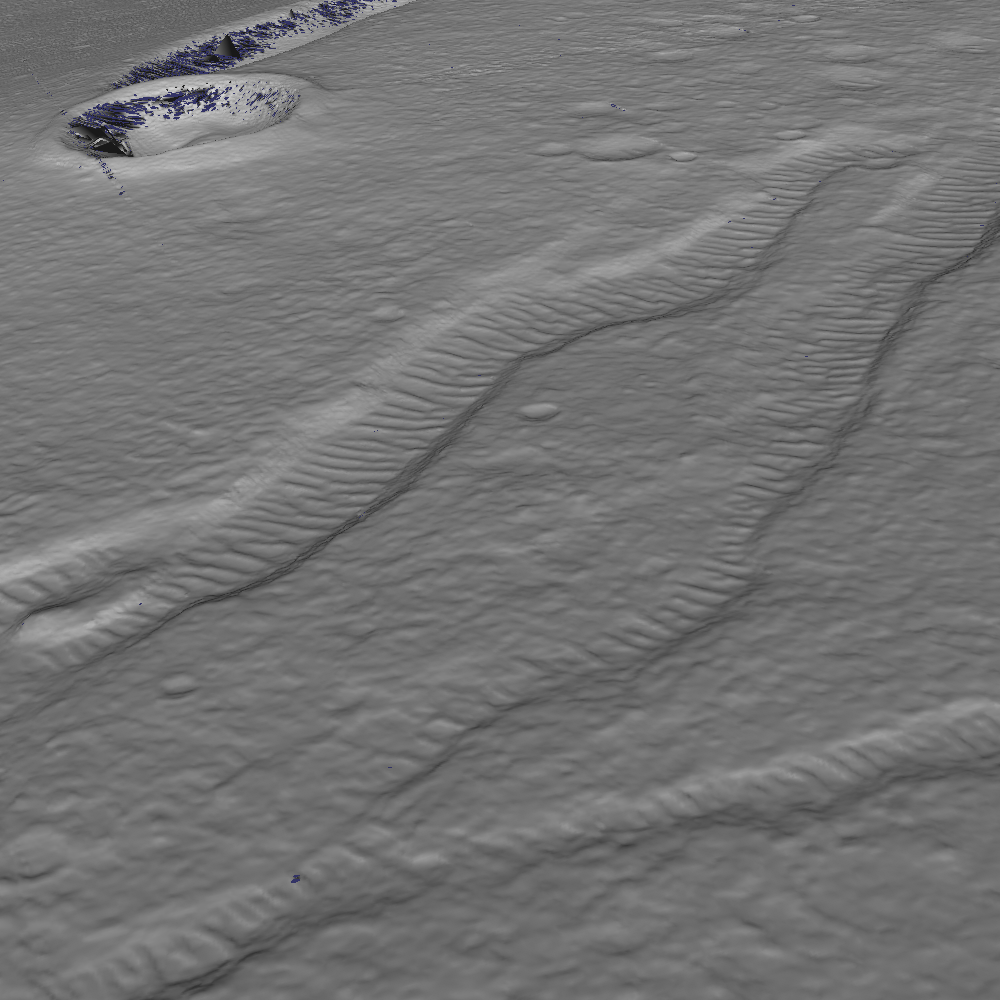
\includegraphics[width=3in]{images/examples/hirise/emare_example.png}}
  \hfil
  \subfigure[{\tt KML Screenshot}]{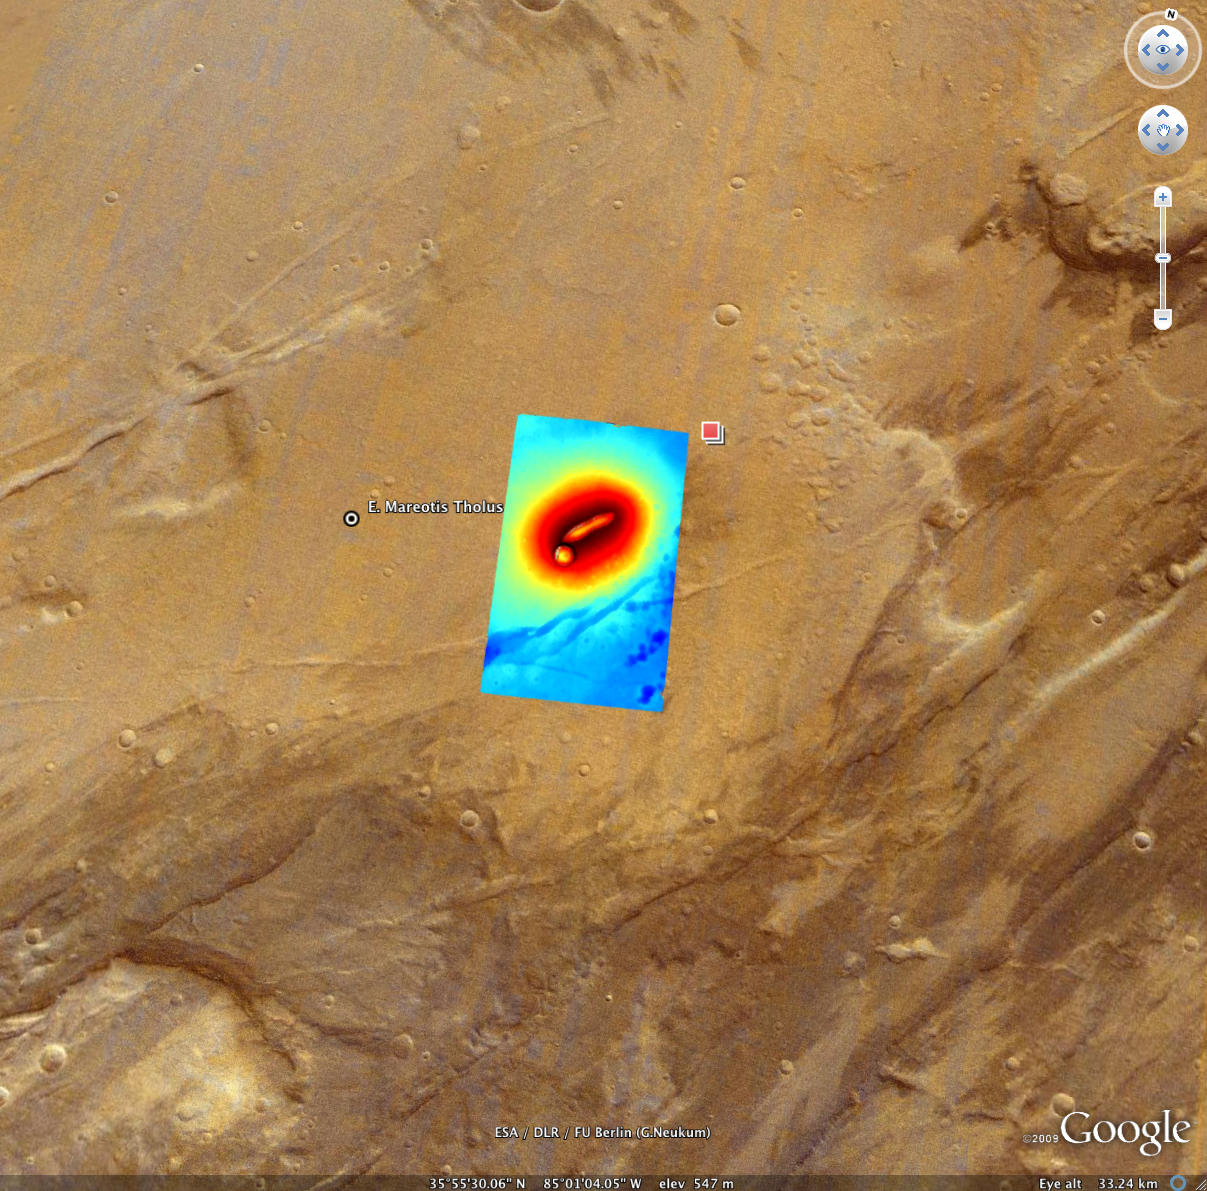
\includegraphics[width=3in]{images/examples/hirise/emare_ge_example.png}}
\caption{Example output using HiRISE data of East Mareotis Tholus.}
\label{fig:hirise_emare_example}
\end{figure}

\subsubsection*{Commands}

\begin{verbatim}
    % Download all of the IMG for PSP_001364_2160 & %
    %                             PSP_001760_2160   %
    ~/HiRISE_stitch.py PSP_001364_2160_RED0_0.IMG
    ~/HiRISE_stitch.py PSP_001760_2160_RED0_0.IMG
    cam2map from=PSP_001364_2160_REDmosaic.norm.cub to=PSP_001364_2160_REDmosaic.map.cub
    cam2map from=PSP_001760_2160_REDmosaic.norm.cub map=PSP_001364_2160_REDmosaic.map.cub ...
            to=PSP_001760_2160_REDmosaic.map.cub matchmap=true
    bandnorm from=PSP_001364_2160_REDmosaic.map.cub to=PSP_001364_2160_REDmosaic.map.norm.cub
    bandnorm from=PSP_001760_2160_REDmosaic.map.cub to=PSP_001760_2160_REDmosaic.map.norm.cub
    ls *.map.norm.cub > fromlist
    ls *1760*.map.norm.cub > holdlist
    equalizer fromlist=fromlist holdlist=holdlist
    rm *REDmosaic.map.norm.cub *REDmosaic.map.cub
    mkdir result
    stereo PSP_001364_2160.map.norm.equ.cub PSP_001760_2160.map.norm.equ.cub result.output
\end{verbatim}

\subsubsection*{Stereo Default}

\begin{verbatim}
    ##      PREPROCESSING      ##

    DO_INTERESTPOINT_ALIGNMENT 0
    DO_EPIPOLAR_ALIGNMENT 0
    INTERESTPOINT_ALIGNMENT_SUBSAMPLING 0
    DO_INDIVIDUAL_NORMALIZATION 0
    FORCE_USE_ENTIRE_RANGE 1

    PREPROCESSING_FILTER_MODE 2
    SLOG_KERNEL_WIDTH 1.5

    ###########################    CORRELATION    ###########################

    H_KERNEL 25
    V_KERNEL 25
    SUBPIXEL_H_KERNEL 25
    SUBPIXEL_V_KERNEL 25

    H_CORR_MIN -80
    V_CORR_MIN -80
    H_CORR_MAX 150
    V_CORR_MAX 50

    SUBPIXEL_MODE 0
    DO_H_SUBPIXEL 1
    DO_V_SUBPIXEL 1

    XCORR_THRESHOLD 2.0
    CORRSCORE_REJECTION_THRESHOLD 1.1

    COST_BLUR 0
    COST_MODE 0

    ############################    FILTERING    ############################

    RM_H_HALF_KERN 5
    RM_V_HALF_KERN 5
    RM_MIN_MATCHES 60 # Units = percest
    RM_THRESHOLD 3
    RM_CLEANUP_PASSES 1

    FILL_HOLES 0

    #############################    DOTCLOUD    ############################

    NEAR_UNIVERSE_RADIUS 0.0
    FAR_UNIVERSE_RADIUS 0.0
\end{verbatim}

\subsection{North Terra Meridiani Crop}

HiRISE website only has to say that this is `Layered Materials within
a Small Crater'. Hopefully you'll still agree that this is cool.

\subsubsection*{Screenshot}

\begin{figure}[h!]
\centering
  \subfigure[{\tt 3D Rendering}]{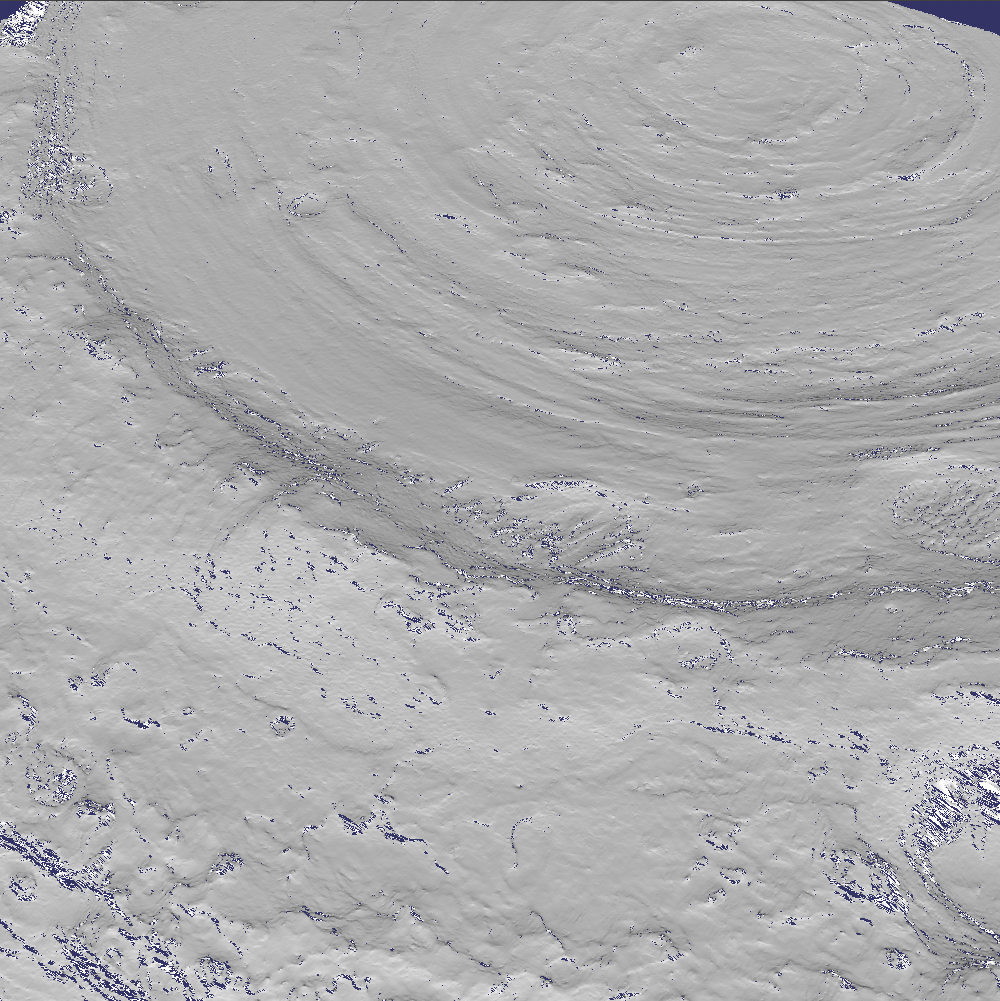
\includegraphics[width=3in]{images/examples/hirise/nterra_example.png}}
  \hfil
  \subfigure[{\tt KML Screenshot}]{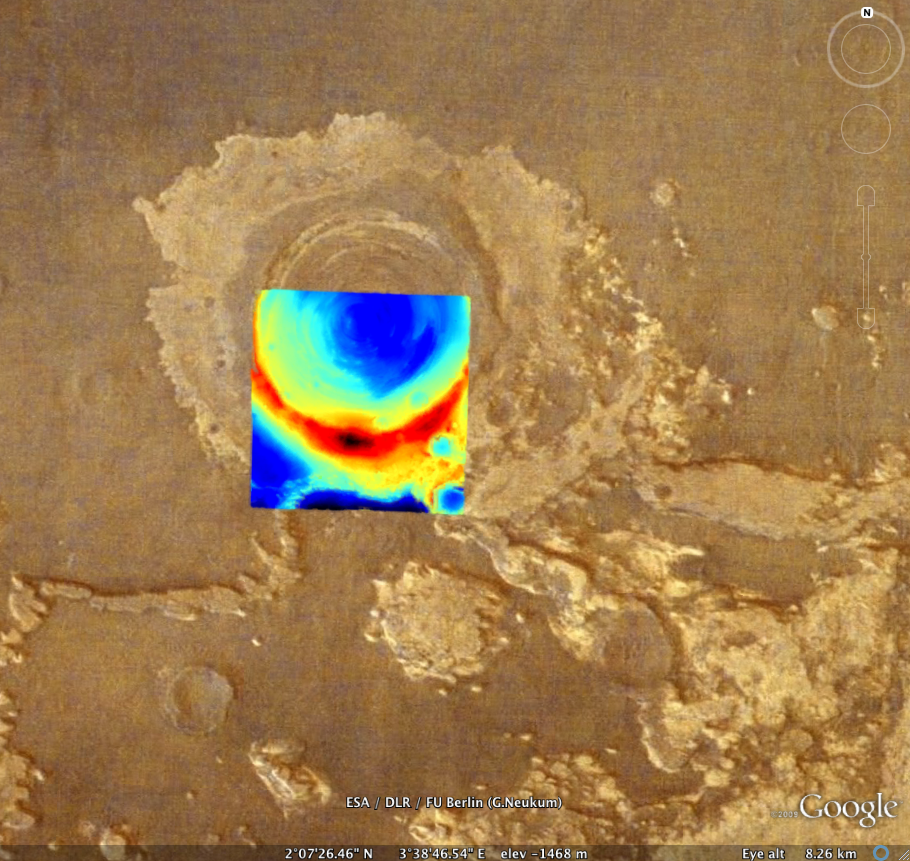
\includegraphics[width=3in]{images/examples/hirise/nterra_ge_example.png}}
\caption{Example output using cropped HiRISE data of North Terra Meridiani.}
\label{fig:hirise_nterra_example}
\end{figure}

\subsubsection*{Commands}

\begin{verbatim}
    % Download all of the IMG for PSP_001981_1825 & %
    %                             PSP_002258_1825   %
    ~/HiRISE_stitch.py PSP_001981_1825_RED0_0.IMG
    ~/HiRISE_stitch.py PSP_002258_1825_RED0_0.IMG
    cam2map from=PSP_001981_1825_REDmosaic.norm.cub to=PSP_001981_1825_REDmosaic.map.cub
    cam2map from=PSP_002258_1825_REDmosaic.norm.cub map=PSP_001981_1825_REDmosaic.map.cub ...
            to=PSP_002258_1825_REDmosaic.map.cub matchmap=true
    bandnorm from=PSP_001981_1825_REDmosaic.map.cub to=PSP_001981_1825_REDmosaic.map.norm.cub
    bandnorm from=PSP_002258_1825_REDmosaic.map.cub to=PSP_002258_1825_REDmosaic.map.norm.cub
    ls *.map.norm.cub > fromlist
    ls *1981*.map.norm.cub > holdlist
    equalizer fromlist=fromlist holdlist=holdlist
    crop from=PSP_001981_1825_REDmosaic.map.norm.equ.cub to=PSP_001981_1825.crop.cub ...
         sample=7497 line=41318 nsamp=10000 nline=10000
    crop from=PSP_002258_1825_REDmosaic.map.norm.equ.cub to=PSP_002258_1825.crop.cub ...
         sample=7982 line=41310 nsamp=10000 nline=10000
    rm *REDmosaic*.cub
    mkdir result
    stereo PSP_001981_1825.crop.cub PSP_002258_1825.crop.cub result/output
\end{verbatim}

\subsubsection*{Stereo Default}

\begin{verbatim}
    ##      PREPROCESSING      ##

    DO_INTERESTPOINT_ALIGNMENT 0
    DO_EPIPOLAR_ALIGNMENT 0
    INTERESTPOINT_ALIGNMENT_SUBSAMPLING 0
    DO_INDIVIDUAL_NORMALIZATION 0
    FORCE_USE_ENTIRE_RANGE 1

    PREPROCESSING_FILTER_MODE 2
    SLOG_KERNEL_WIDTH 1.5

    ###########################    CORRELATION    ###########################

    H_KERNEL 45
    V_KERNEL 45
    SUBPIXEL_H_KERNEL 25
    SUBPIXEL_V_KERNEL 25

    H_CORR_MIN -270
    H_CORR_MAX -70
    V_CORR_MIN -14
    V_CORR_MAX 26

    SUBPIXEL_MODE 0
    DO_H_SUBPIXEL 1
    DO_V_SUBPIXEL 1

    XCORR_THRESHOLD 2.0
    CORRSCORE_REJECTION_THRESHOLD 1.2

    COST_BLUR 21
    COST_MODE 2

    ############################    FILTERING    ############################

    RM_H_HALF_KERN 5
    RM_V_HALF_KERN 5
    RM_MIN_MATCHES 60 # Units = percest
    RM_THRESHOLD 3
    RM_CLEANUP_PASSES 1

    FILL_HOLES 1

    #############################    DOTCLOUD    ############################

    NEAR_UNIVERSE_RADIUS 0.0
    FAR_UNIVERSE_RADIUS 0.0
\end{verbatim}

\section{MESSENGER MDIS}

This a proof of concept showing of the strength of building on top of
ISIS. MDIS data is not a goal for the designers but it does have a
camera model in ISIS. This alone means that it too can be processed by
the Ames Stereo Pipeline.

For future mappers it is suggested checking out Mercury Flyby 3 data
which was not available at the time of this writing. Flyby 3 and Flyby
2 seem to have covered some of the same terrain with the narrow angle
camera.

\subsection{Wide Angle on flyby 2}

Like most imagery coming from spacecraft that are currently not in
orbit with their target, it is very hard to find good stereo
pairs. This is taken from a single flyby from the same camera seconds
apart. It should also be noted that this pair is taken from different
wave lengths as well \emph{(The letter at the end of the file
  designates the current filter being used on the wide angle
  camera)}. Unfortunately theres not enough of a perspective change to
make anything other than the spherical surface.

\subsubsection*{Screenshot}

\begin{figure}[h!]
  \begin{center}
  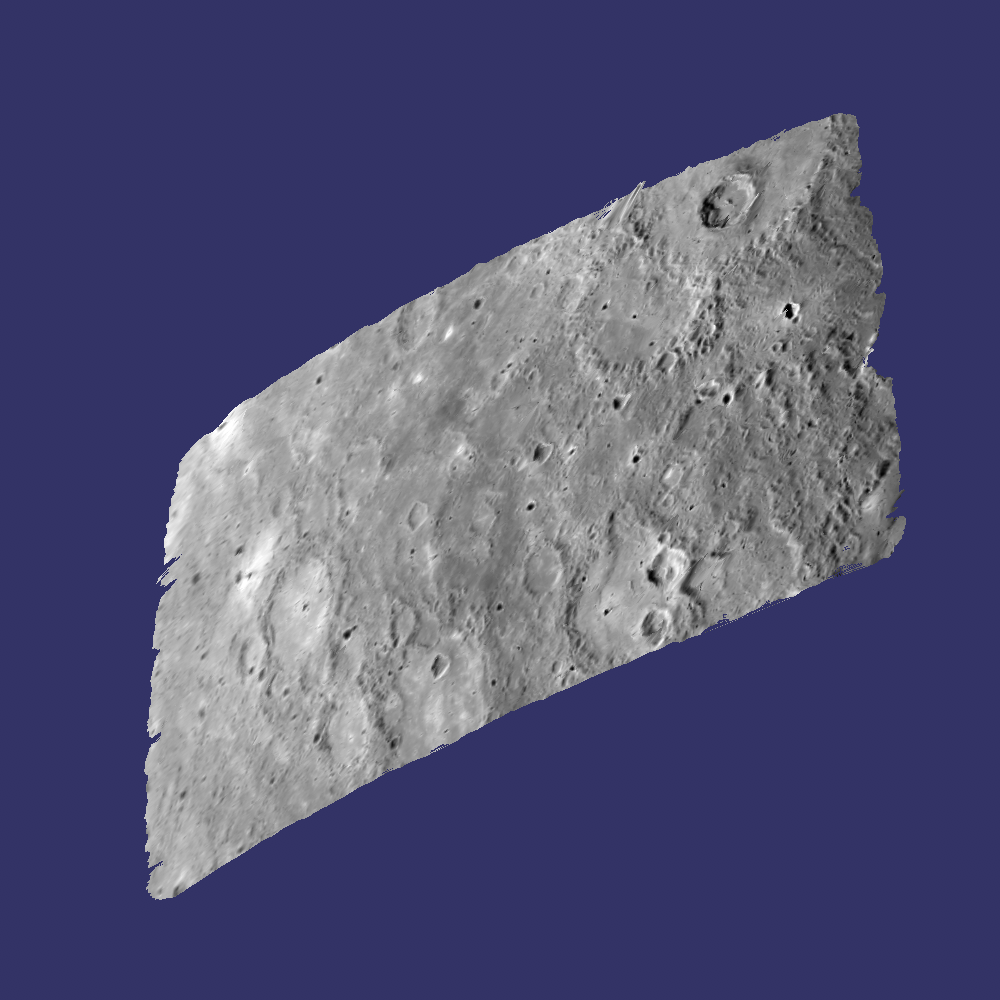
\includegraphics[width=5in]{images/examples/mdis/mdis_wide_example.png}
  \end{center}
  \caption{ A rough attempt at MDIS imagery }
  \label{fig:mdis_attempt}
\end{figure}

\subsubsection*{Commands}

\begin{verbatim}
    mdis2isis from=EW0108825359A.IMG to=EW0108825359A.cub
    mdis2isis from=EW0108825379C.IMG to=EW0108825379C.cub
    spiceinit from=EW0108825359A.cub
    spiceinit from=EW0108825359C.cub
    ipfind --max 10000 *.cub
    ipmatch -i 10 -r homography *.cub
    mkdir result
    stereo EW0108825359A.cub EW0108825379C.cub stereo/output
\end{verbatim}

\subsubsection*{Stereo Default}

\begin{verbatim}
    ##      PREPROCESSING      ##

    DO_INTERESTPOINT_ALIGNMENT 1
    DO_EPIPOLAR_ALIGNMENT 0
    INTERESTPOINT_ALIGNMENT_SUBSAMPLING 0
    DO_INDIVIDUAL_NORMALIZATION 1
    FORCE_USE_ENTIRE_RANGE 0

    PREPROCESSING_FILTER_MODE 2
    SLOG_KERNEL_WIDTH 1.5

    ###########################    CORRELATION    ###########################

    H_KERNEL 25
    V_KERNEL 25
    SUBPIXEL_H_KERNEL 19
    SUBPIXEL_V_KERNEL 19

    H_CORR_MIN -10
    H_CORR_MAX 10
    V_CORR_MIN -2
    V_CORR_MAX 2

    SUBPIXEL_MODE 2
    DO_H_SUBPIXEL 1
    DO_V_SUBPIXEL 1

    XCORR_THRESHOLD 2.0
    CORRSCORE_REJECTION_THRESHOLD 1.3

    COST_BLUR 5
    COST_MODE 0

    ############################    FILTERING    ############################

    FILL_HOLES 1

    RM_H_HALF_KERN 5
    RM_V_HALF_KERN 5
    RM_MIN_MATCHES 60 # Units = percent
    RM_THRESHOLD 3

    #############################    DOTCLOUD    ############################

    NEAR_UNIVERSE_RADIUS 0.0
    FAR_UNIVERSE_RADIUS 0.0

\end{verbatim}
